\documentclass[submit,techreq,noauthor]{eco}	% semi style
\usepackage[dvips]{graphicx}
\usepackage{listings, jlisting} 		% for source code
\usepackage{url}
\usepackage{setspace}
\usepackage{here}
%\setstretch{1.5} % 行間を広くします(資料チェックしてもらうときはコメントを外す)

\lstset{
  basicstyle={\ttfamily},
  identifierstyle={\small},
  commentstyle={\smallitshape},
  keywordstyle={\small\bfseries},
  ndkeywordstyle={\small},
  stringstyle={\small\ttfamily},
  frame={tb},
  breaklines=true,
  columns=[l]{fullflexible},
  numbers=left,
  xrightmargin=0zw,
  xleftmargin=3zw,
  numberstyle={\scriptsize},
  stepnumber=1,
  numbersep=1zw,
  lineskip=-0.5ex
}

\begin{document}

\semino {5/5}					% 年度/回数
\date   {5/04/25/火}				% 平成/月/日/曜日
\title  {共有ライブラリを置き換える\\Linuxマルウェア:Symbioteの調査}	% タイトル
\author {奥 若菜}				% 氏名


\begin{abstract}
	Linuxにおいて,プログラム実行時に共有ライブラリを動的リンクするために使用する環境変数にLD\_PRELOADがある.
  2021年に発見されたSymbioteは,LD\_PRELOADを使用して,すべての実行中のプロセスにロードされる共有ライブラリとして動作し,
  正当なプロセスの下で自身や他のマルウェアの痕跡を隠蔽する.
  本研究では,Symbioteのような,共有ライブラリを用いたDynamic Linker Hijackingを行うマルウェアを動的解析し,その挙動を明らかにするとともに,効果的な検知手法の発見を目指す.
\end{abstract}
\maketitle


\section{はじめに}
近年,IoTデバイスの普及や企業のクラウドシフトにより,Linuxマシン上で動作するマルウェアが増加している\cite{TREND-MICRO}.
Linuxマシンの中にはサーバとして定常稼働しており,固定のIPアドレスが割り振られているものも多く,攻撃インフラとしての利用価値が高いことから,今後もLinuxマシンを標的とするマルウェアは増加すると予想される.

2021年に発見されたSymbioteは,Linuxで一般的に見られるマルウェアとは異なる特徴を持ち,極めて検出が困難とされる\cite{Symbiote}.
Symbioteは,単独の実行可能ファイルではなく,LD\_PRELOADによってすべての実行中のプロセスにロードされる共有ライブラリとして動作する.
LD\_PRELOADとは,Linuxにおいて,プログラム実行時に共有ライブラリを動的リンクするために使用される環境変数である.
Symbioteは,LD\_PRELOADを使用することで,プログラムによって要求される正当な共有ライブラリの代わりに,悪意のある共有ライブラリを提供する.
このように悪意のある共有ライブラリをプログラムにロードし,不正なコードを実行する攻撃をDynamic Linker Hijackingという\cite{MITRE-ATT&CK}.
この攻撃では正当なプロセスの下で実行がマスクされるため,プロセスベースの解析は回避される可能性が高い.

本研究は,動的解析を行うことによってSymbioteの挙動を明らかすることを目指す.
また,SymbioteのようなDynamic Linker Hijackingを行うLinuxマルウェアの効果的な検知手法および対策方法を考察する.


以下,2章でSymbioteの機能を説明し,3章で静的解析によって得られた検体の詳細な設計を説明する.
4章で検体を用いた動的解析の結果を述べ,5章でまとめる.\\


\section{Symbioteの機能}
Symbioteが初めて検知されたのは2021年11月であり,
ラテンアメリカの金融セクターを標的とするために作成されたとされている.
Symbioteについての調査は,Intezerの研究者Joakim KennedyとBlackBerryのResearch and Intelligence Teamによって
行われ,レポートが作成されている.以下に文献\cite{Symbiote}のレポートをもとにSymbioteの機能を示す.


\subsection{検知回避機能}
Symbioteは,LD\_PRELOADで指定した共有ライブラリによって,プログラムによる関数の呼び出しをフックし,
悪意のあるコードを実行することで,検知を回避する.具体的には,C言語の標準ライブラリであるlibcおよび
パケットキャプチャのためのライブラリであるlibpcapの関数をフックすることで,以下のような回避機能を実現する.
  \begin{description}
    \item [プロセスの隠蔽] \mbox{}\\
    呼出し元のアプリが/proc以下にあるファイルまたはディレクトリにアクセス
    しようとすると,プロセス名を元に出力を消去する.
    \item [ファイルの隠蔽] \mbox{}\\
    呼出し元のアプリが上記以外の場所にアクセスしようとすると,暗号化さ
    れたファイルリストにある名前を元に出力を消去する.
    \item [ネットワークトラヒックの隠蔽] \mbox{}
      \begin{description}
        \item[UDP:] 
        libpcapの関数をフックし,受信したパケットごとにドメインの文字列をチェックする.一致した場合はそのパケットをスキップして呼出し元に返す.
        \item[TCP:] 
        fopenとfopen64をフックし,プロセスがproc/net/tcpを開こうとすると,該当するポートをスキップして呼出し元に返す.
        感染マシンがeBPFを使用してパケットキャプチャを行う場合は,setsockoptをフックし,提供されたeBPFコードの前に独自のバイトコードを付加することで,ポートに基づきパケットを消去する.
      \end{description}
  \end{description}

\subsection{ルートキット機能}
Symbioteはすべての実行中のプロセスに感染した後,認証情報の収集し,攻撃者にリモートアクセスなどのルートキット機能を提供する.

認証情報の収集は,sshやscapプロセスによって呼び出されるlibcのread関数をフックすることで行われる.
収集した認証情報はファイルに書き込まれるだけでなく,
16進エンコードされ,攻撃者が運用するサーバにDNSのAレコード要求を通じて持ち出される.\\
\indent
感染したマシンへのリモートアクセスは,Pluggable Authentication
Module(PAM)機能をフックすることで提供される.アプリケーション(telnetやssh)がPAMを利用してユーザを認証する際に,攻撃者のあら
かじめ設定したものと同じ認証情報でアクセスすると,フックされた関数が成功応答を返すとともに,攻撃者もアクセスが可能になる.

\subsection{緊急アクセス機能}
Symbioteは通常のプロセスが機能しない場合に,攻撃者のC\&CサーバにDNSのTXTレコード要求を送信し,マシンへの緊急アクセスを
提供する.TXTレコードの形式は,\%MACHINEID\%.\%C\&C\_DOMAIN\%となっている.応答を取得すると,このマルウェアはコンテンツをbase64
デコードし,コンテンツが正しいed25519秘密鍵で署名されているかどうかをチェックし,
RC4でコンテンツを復号して,生成されたbashプロセスでシェルスクリプトを実行する.\\


\section{検体の静的解析による設計の調査}
2章では,文献\cite{Symbiote}のレポートで示されているSymbioteの機能を紹介した.
ただし,このレポートはSymbioteで一般的に見られる機能を紹介しており,具体的な検体の情報は明記されていない.
また,その他の文献についても,検体ごとの詳細な情報を示すものは見つかっていない.
\indent
Symbioteでは,複数の検体において類似した機能が見られることが示されているが,検体が提供するライブラリ関数や,隠蔽されるファイル・プロセスの名前はそれぞれの検体で異なる.
Symbioteのそれぞれの検体について静的解析を行い,詳細な設計を明らかにする.

\subsection{検体}
Intezer AnalyzeとVirusTotalを用いてSymbioteを探索したところ,表\ref{table: Artifact}に示す6検体が見つかった.
これらはIntezerのレポートに記載されている検体のハッシュと一致しており,更新情報もないため,現在までで見つかっている検体は,この6検体が全てである可能性が高い.\\
\indent
6検体のうち,検体4のみが実行ファイルであり,実行を開始すると2.3章で述べた緊急アクセス機能を提供する.
その他の検体は,すべて共有ライブラリファイルであり,LD\_PRELOADに検体ファイルのパスを代入することで動作する.\\
\indent
現在までで静的解析を行ったのは,Symbioteの初期開発ビルドである検体1と,最も新しく発見された検体6である.この2つの検体について解析結果を示す.

\begin{table}[H]
  \caption{Symbioteの検体一覧}
  \label{table: Artifact}
  \centering
  \begin{tabular}{|l|l|l|}
  \hline
  No. & Hash                                                                                                        & First Seen \\ \hline
  1   & \begin{tabular}[c]{@{}l@{}}121157e0fcb728eb8a23b55457e89d45\\ d76aa3b7d01d3d49105890a00662c924\end{tabular} & 2021/11/27 \\ \hline
  2   & \begin{tabular}[c]{@{}l@{}}f55af21f69a183fb8550ac60f392b05d\\ f14aa01d7ffe9f28bc48a118dc110b4c\end{tabular} & 2022/01/19 \\ \hline
  3   & \begin{tabular}[c]{@{}l@{}}ec67bbdf55d3679fca72d3c814186ff4\\ 646dd779a862999c82c6faa8e6615180\end{tabular} & 2022/01/26 \\ \hline
  4   & \begin{tabular}[c]{@{}l@{}}45eacba032367db7f3b031e5d9df10b\\ 30d01664f24da6847322f6af1fd8e7f01\end{tabular} & 2022/01/29 \\ \hline
  5   & \begin{tabular}[c]{@{}l@{}}a0cd554c35dee3fed3d1607dc18debd\\ 1296faaee29b5bd77ff83ab6956a6f9d6\end{tabular} & 2022/02/01 \\ \hline
  6   & \begin{tabular}[c]{@{}l@{}}cb4bbe3af754779e673c6ae84cb38d7f\\ 2ccbc9a1d59c52abbb98451d070dba3c\end{tabular} & 2022/08/19 \\ \hline
  \end{tabular}
\end{table}


\subsection{検体1の解析結果}
\subsubsection{ライブラリ関数}
実行中のプロセスに提供されるライブラリ関数と,それらの呼出し関係に注目して静的解析を行った.
検体1によって提供される13個のライブラリ関数と,その機能を以下にまとめる.
これらの関数は,libcなどのライブラリ関数と同様の機能を提供しつつ,隠蔽や認証情報の収集,攻撃者との通信を行う.
\begin{description}

  \item [プログラムの初期化・終了処理] \mbox{}
  \begin{description}
    \item[\_init:] プログラムの初期化処理を行う.
    \item[call\_gmon\_start:] プログラム実行性能を計測する.
    \item[\_fini:]プログラムの終了処理を行う.
  \end{description}

  \item [TCP通信・ファイル・プロセスの隠蔽] \mbox{}
  \begin{description}
    \item[fopen・fopen64:] ファイルを開く.隠蔽するポートの内容はファイルに書き込まない.
    \item[readdir・readdir64:] ディレクトリエントリを返す.隠蔽するファイルとプロセスはNULLを返す.
  \end{description}

    \item [認証情報の収集] \mbox{}
  \begin{description}
    \item[pam\_authenticate:] PAMを使用してユーザ認証を行う.ユーザ名やパスワードを収集する.
    \item[readdir・readdir64:] PAM項目の値を更新する.PAM項目がパスワードなら保存する.\\
  \end{description}

  \item [キーロギング・通信・暗号化] \mbox{}
  \begin{description}
    \item[read:] コマンドラインの情報とホストのIPアドレスを収集し,攻撃者に送信する.
    \item[recvmsg:]ソケットからデータを受信する.ポートや文字列に基づいて隠蔽する.
    \item[crc32b:] crc32のハッシュ値を返す.
    \item[RC4:] RC4で文字列の暗号化を行う.\\
  \end{description}
\end{description}

\subsubsection{関数の呼出し関係}
検体1によって実行中のプロセスに提供されるのは3.2.1節で示した13個のライブラリ関数のみである.
しかし,検体の挙動を明らかにするためには,それらのライブラリ関数によって二次的に呼び出される関数も調査する必要がある.\\
\indent
例えば,検体1が提供するreaddirは図\ref{fig:call-graph}のように関数呼出しを行っている.呼出される関数のうち,
check\_proc,hidden\_proc,hidden\_fileは,readdirと同様に検体1によって実装された関数であり,プロセスやファイルの隠蔽のために使用される.
一方で,dlsymとstrcmpはlibcライブラリによって提供され,特にdlsymはlibcで定義される本来のreaddirを呼び出すために使用される.\\
\indent
検体1で実装される全ての関数と,それらの呼出し関係は付録に記載する.

\begin{figure}[H]
	\centering
  \fbox{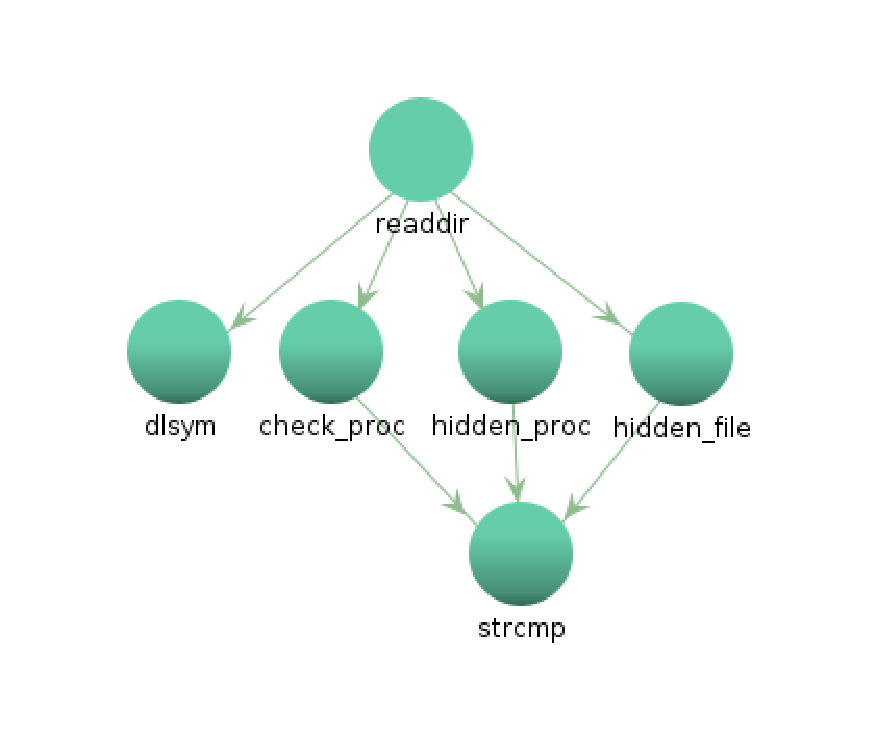
\includegraphics[width=7cm]{fig/call-graph.eps}}
	\caption{readdirの呼出し関係}
	\label{fig:call-graph}
\end{figure}

\subsubsection{隠蔽されるファイル・プロセスの名前}
プロセスやファイルの隠蔽のために使用される関数であるhidden\_proc,hidden\_fileが参照するアドレスを調べることで,
検体1によって隠蔽されるファイル名とプロセス名を特定することができた.以下にそれらを示す.
\begin{description}
  \item[隠蔽されるプロセス] 
  \begin{itemize}
    \item kernelconfig
    \item kerneldev
    \item threadmulti
  \end{itemize}
  \item[隠蔽されるファイル] 
  \begin{itemize}
    \item kernelconfig
    \item kerneldev
    \item threadmulti
    \item usb.h
    \item kerneldev.so 
  \end{itemize}
\end{description}

\subsection{検体6の解析結果}
検体6は,多数の関数によって関数rc4が呼び出されるように設計されており,
隠蔽するファイル名やプロセス名,収集した認証情報など,ほとんどの文字列がRC4で暗号化されていることが分かった.
そこで,rc4に渡されるポインタから暗号化キーを特定し,暗号化された文字列を復号するプログラムを作成した.
これにより,隠蔽されるファイル名とプロセス名を定義する文字列を復号することができた.以下にそれらを示す.
\begin{description}
  \item[隠蔽されるプロセス] 
  \begin{itemize}
    \item \lbrack watchdos/0\rbrack
    \item dbus
    \item java8
    \item \lbrack kswapd1\rbrack
  \end{itemize}
  \item[隠蔽されるファイル] 
  \begin{itemize}
    \item mprfx.so
    \item dbus
    \item .db.inc.php
    \item libpcap3.so
    \item kswapd\\
  \end{itemize}
\end{description}

\section{検体の動的解析}
検体1を隔離環境で実行し,システムコールトレースとライブラリコールトレースを行った.\\
\indent
4.1節で解析環境について説明し,4.2節でシステムコールトレースの結果を示す.
4.3節でライブラリコールトレースの結果を示し,4.4節で検体の動的解析についての考察を述べる.

\subsection{解析環境}
解析環境を構成するソフトウェアを表2に示す.
ゲストOSからホストおよびネットワークへのアクセスはできない.
また,検体の実行と解析は全てゲストOS上で行う.

\begin{table}[H]
  \caption{解析環境}
  \label{table: 解析環境}
  \centering
  \begin{tabular}{|l|l|}
  \hline
  Guest OS   & Ubuntu 22.04.2 LTS \\ \hline
  emulator   & QEMU 6.2.0         \\ \hline
  hypervisor & KVM                \\ \hline
  Host OS    & Ubuntu 22.04.2 LTS \\ \hline
  \end{tabular}
\end{table}


\subsection{システムコールトレースの結果}
検体1をLD\_PRELOADに設定し,lsコマンドでディレクトリ内のファイルを表示したときのシステムコールをstraceコマンドで取得する.
一方は中身が空のディレクトリ,
もう一方は隠蔽されるファイルが1つのみ存在するディレクトリに対して,それぞれlsコマンドを実行した.\\
\indent
これらのシステムコールを比較したところ,
どちらもシステムコールの合計呼出し数は102回で,順序や種類も同じであった.
また,ファイルの隠蔽に直接関係するようなシステムコールも確認できなかった.

\subsection{ライブラリコールトレースの結果}
検体1をLD\_PRELOADに設定した状態で,ディレクトリのエントリを読み込むだけのプログラムtest-readdir.cを実行し,
ltraceコマンドで動的リンクされる関数を取得した\lbrack 図\ref{fig:ltrace}\rbrack.

\begin{figure}[H]
	\centering
  \fbox{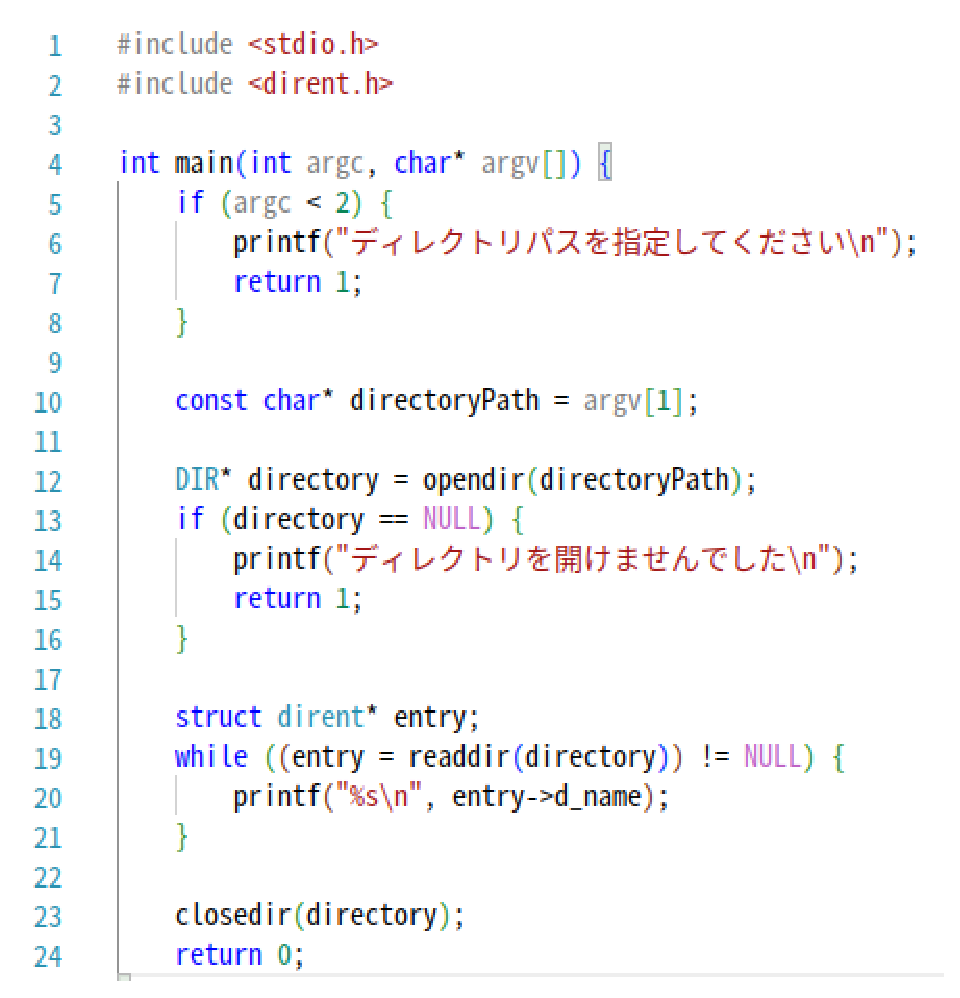
\includegraphics[width=8cm]{fig/readdir.eps}}
	\caption{test-readdir.cに動的リンクされる関数}
	\label{fig:readdir}
\end{figure}

\begin{figure}[H]
	\centering
  \fbox{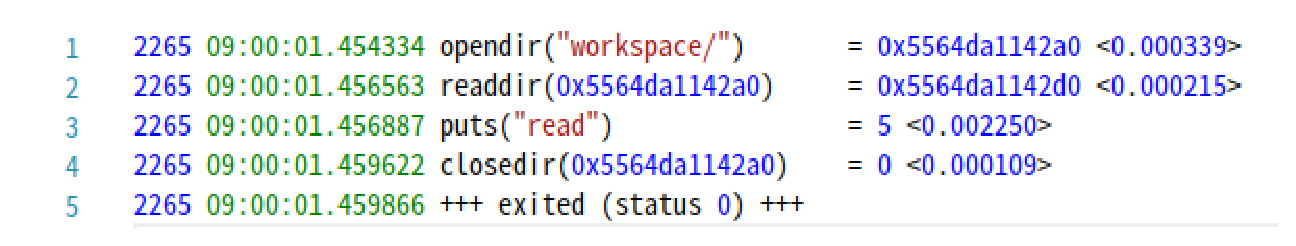
\includegraphics[width=8cm]{fig/ltrace.eps}}
	\caption{test-readdir.cに動的リンクされる関数}
	\label{fig:ltrace}
\end{figure}

\subsection{検体の実行結果}
表1に示した6検体をそれぞれ実行した結果,No.3以外の検体ではSegmentation Faultが発生したため,動作が確認できたのはNo.3のみであった.
ここではNo.3の動的解析の結果について述べる.

実行を開始すると,マルウェアは/etc/resolv.confで設定されているローカルDNSサーバ(127.0.0.53)にDNSのTXTレコード要求を送信する.
ローカルDNSサーバは外部のDNSサーバへ名前解決要求を試みるが,ネットワークに接続されていないため,到達することができない.そのため図1のように”DNS: RCODE\_SERVER\_FAILURE”というエラーメッセージが出力され,タイムアウトにより実行が終了する.

\begin{figure}[H]
	\centering
  \fbox{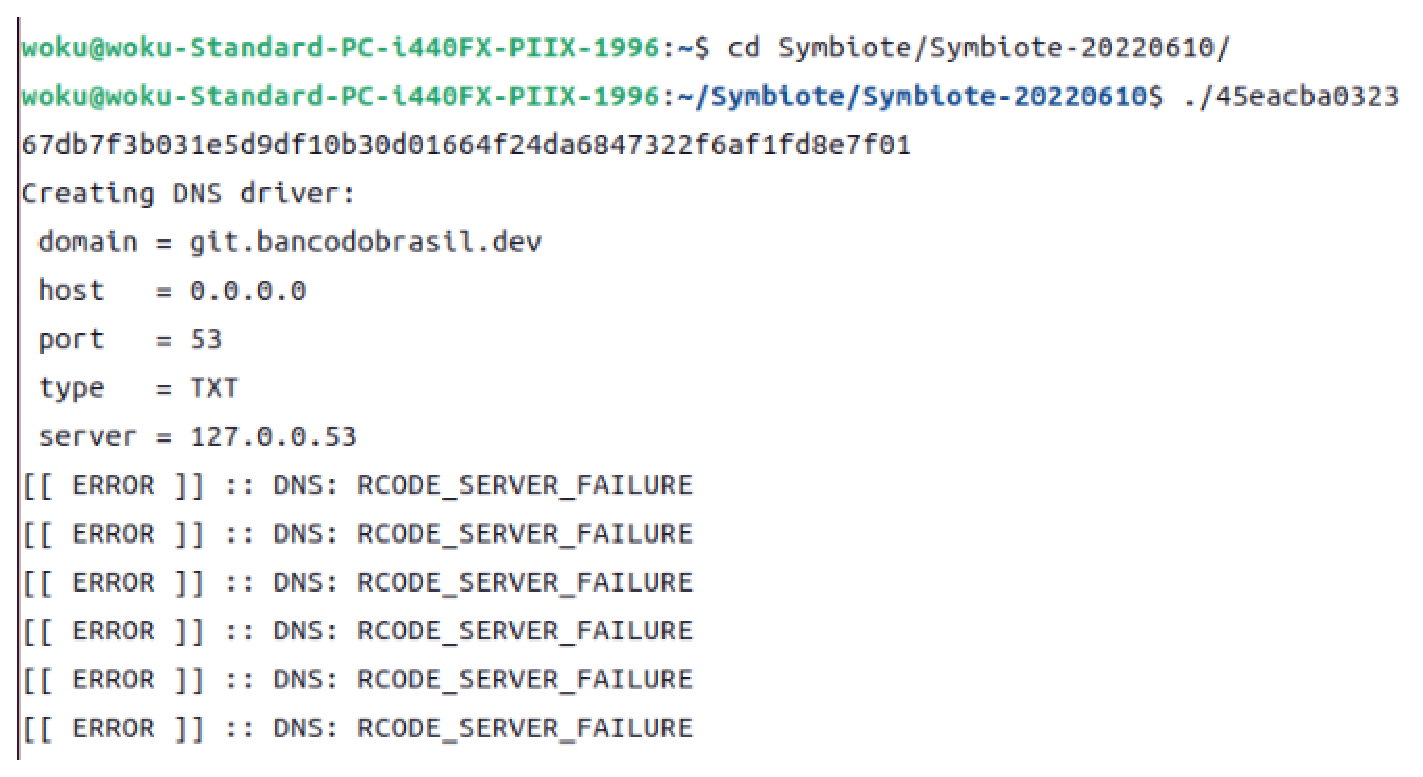
\includegraphics[width=8cm]{fig/001.eps}}
	\caption{実行結果(DNS応答なし)}
	\label{fig:001}
\end{figure}

\subsection{DNS応答を行った場合の検体の実行結果}
マルウェアを継続して動作させるためには,DNSサーバへの接続を行い,TXTレコード要求に応じる必要があると考えられる.検体が動作する環境は,ネットワークに接続していないため,外部のDNSサーバを使用することはできない.
そこで,ゲストOSのローカルポート127.0.0.1:53にDNSサーバ(ns.bancodobrasil.dev)を構築し,マルウェアへの応答を行う.

図2のパケットログより,マルウェアがDNS要求をおこなうFQDNは,リクエストごとに頭の4文字が異なることがわかる.
また,FQDNの構成は,16進エンコードされた文字列に,”git.bancodobrasil.dev”というドメインが続く形式となっている.
\begin{figure}[H]
	\centering
  \fbox{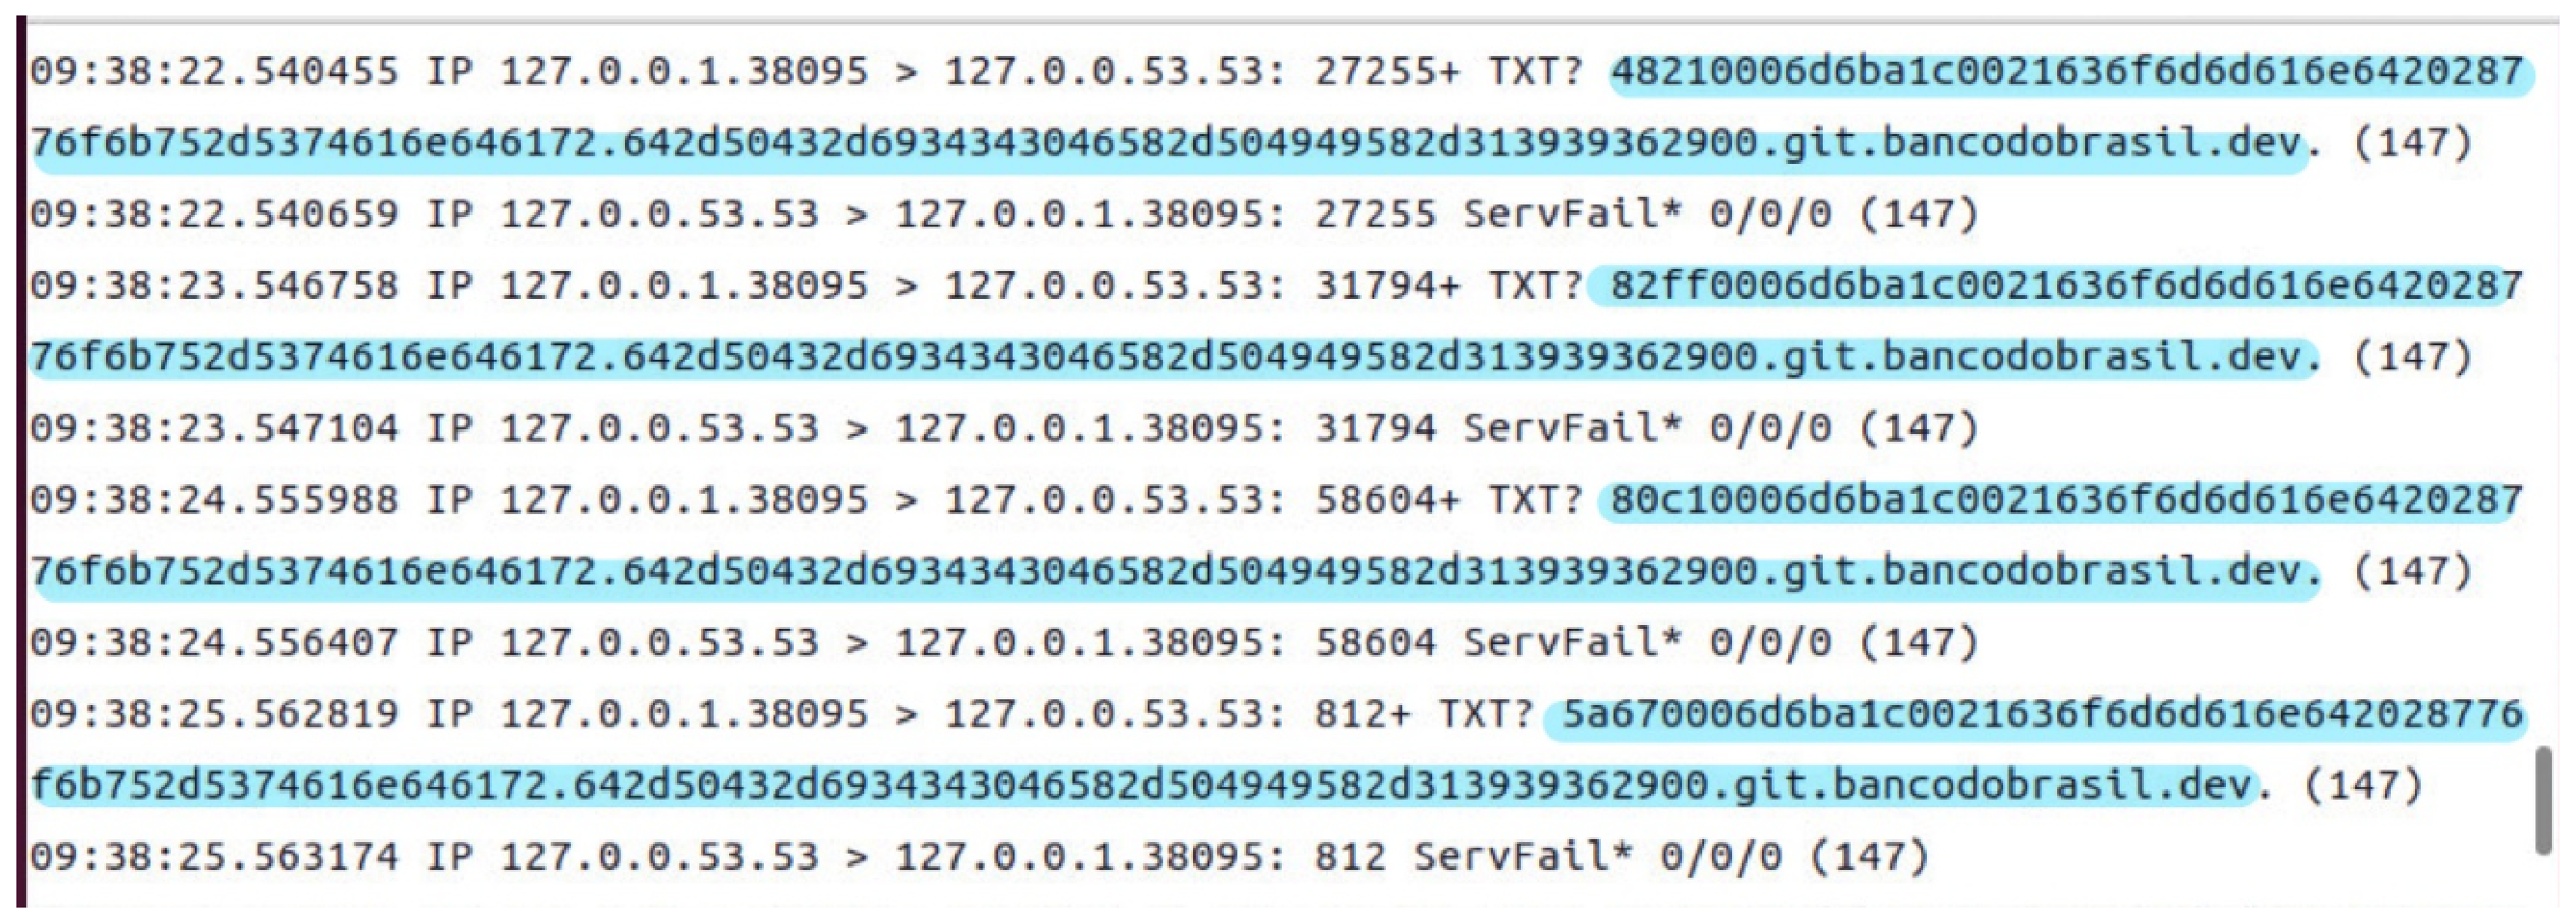
\includegraphics[width=8cm]{fig/002.eps}}
	\caption{パケットログ}
	\label{fig:packet}
\end{figure}

さらに16進でエンコードされた文字列をデコードすると,”command (woku-Standard-PC-i440FX-PIIX-1996)”という文字列が含まれることがわかる.
これは,マルウェアを実行したゲストOSのマシンIDと一致する.\\

FQDNの冒頭4文字は毎リクエストごとに異なることを踏まえ,ワイルドカードDNSレコードを使用して,DNSサーバ(ns.bancodobrasil.dev)のゾーン情報を表3のように設定した.
なお,TXTレコードの値には適当な16進数の文字列"68656c6c6f"(hello)を設定した.

\begin{table}[H]
  \centering
  \caption{DNSサーバ ゾーン情報}
  \label{table: ゾーン情報}
  \begin{tabular}{|l|l|l|l|}
  \hline
  hostname                                                                                                             & class & type & value                                                            \\ \hline
  bancodobrasil.dev.                                                                                                   & IN    & NS   & \begin{tabular}[c]{@{}l@{}}ns.bancodo\\ brasil.dev.\end{tabular} \\ \hline
  ns.bancodobrasil.dev.                                                                                                & IN    & A    & 127.0.0.1                                                        \\ \hline
  \begin{tabular}[c]{@{}l@{}}*.642d50432d6934343046\\ 582d504949582d3139393\\ 62900.git.bancodobrasil.dev\end{tabular} & IN    & TXT  & "68656c6c6f"                                                     \\ \hline
  \end{tabular}
\end{table}

  実行結果は図3のようになった.DNSのTXTレコード要求に応じることができたが,正しい値で応答していないため,"Tried to access a non-existent session(controller\_data\_incoming)"
  というエラーメッセージが出力され,タイムアウトによりマルウェアの実行が停止した.

  \begin{figure}[H]
    \centering
    \fbox{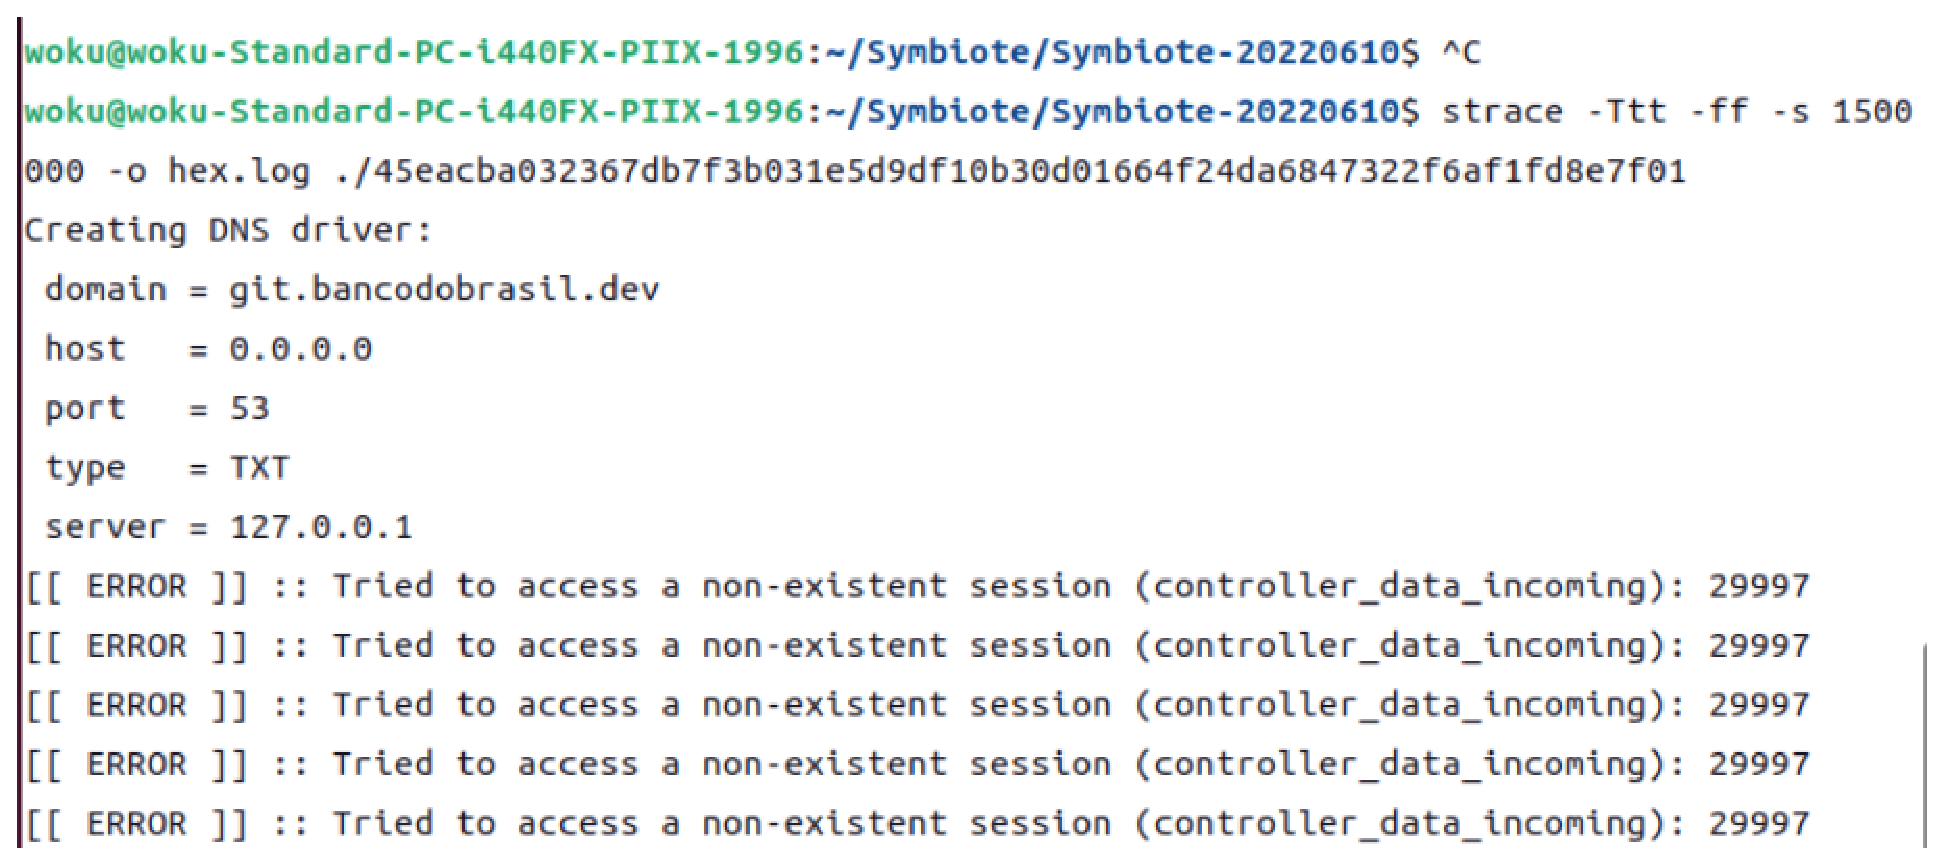
\includegraphics[width=8cm]{fig/003.eps}}
    \caption{実行結果(DNS応答あり)}
    \label{fig:003}
  \end{figure}

\subsection{考察}
No.3の検体は実行とともにDNSのTXTレコード要求を攻撃者のC2サーバに送信し,その出力やパケットが隠蔽されている様子は確認できなかった.
これらの特徴は,Symbioteの調査レポートにおける,緊急アクセス機能の特徴と一致する.よって,このマルウェアの通常プロセスは機能していない可能性が高い.
  また,DNSのTXTレコード要求に対しての応答には,攻撃者の署名が必要ということになり,これ以上の実行は困難であると考えられる.\\

\section{おわりに}
LD\_PRELOADを利用することで,共有ライブラリの置き換えを行うLinuxマルウェアである
Symbioteの調査と,その検体の動的解析を行った.結果として,現在入手している検体は
共有ライブラリの置き換えによる検知回避機能を実行する可能性が低いことがわかった.
検知が困難とされるLinuxマルウェアの効果的な解析手法を発見するために,Symbioteのような機能をもつ
他のマルウェアについても調査していく必要がある.

%bibtex
\setlength\baselineskip{12pt}
{\small
	\bibliography{references}
	\bibliographystyle{ipsjunsrt}
}


\end{document}
